\chapter{Istruzioni all'uso}
Il seguente capitolo fornirà tutte le spiegazioni per il corretto utilizzo del prodotto.

\section{Home}
Questa è la prima schermata disponibile del prodotto. Qui è possibile caricare i dati sotto forma di dataset o di sessione salvata in precedenza.

\begin{figure}[H]
    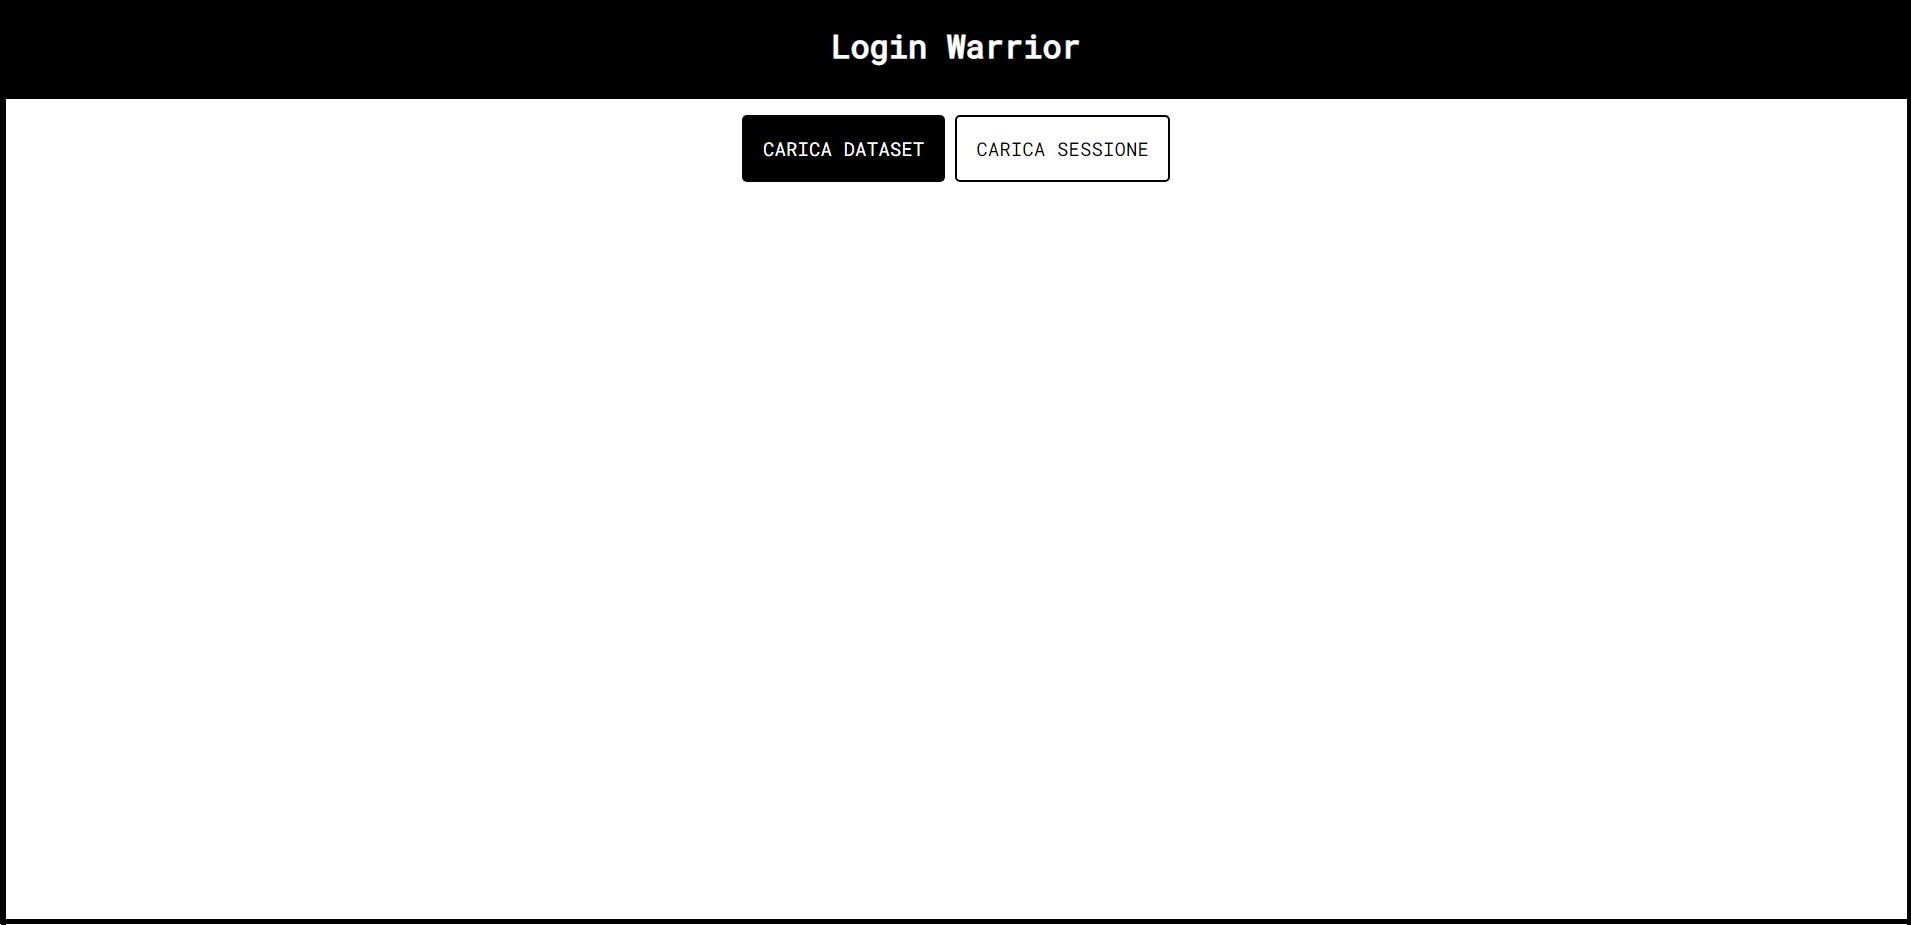
\includegraphics[width=1.0\textwidth]{Home.jpg}
    \caption{Screenshot della Home}
\end{figure}

\subsection{Carica dataset}
Cliccando su "Carica dataset" comparirà una finestra di dialogo che ci permetterà di caricare il dataset. Seleziona quindi il file desiderato e poi clicca su "Apri" per caricare il file.

\begin{figure}[H]
    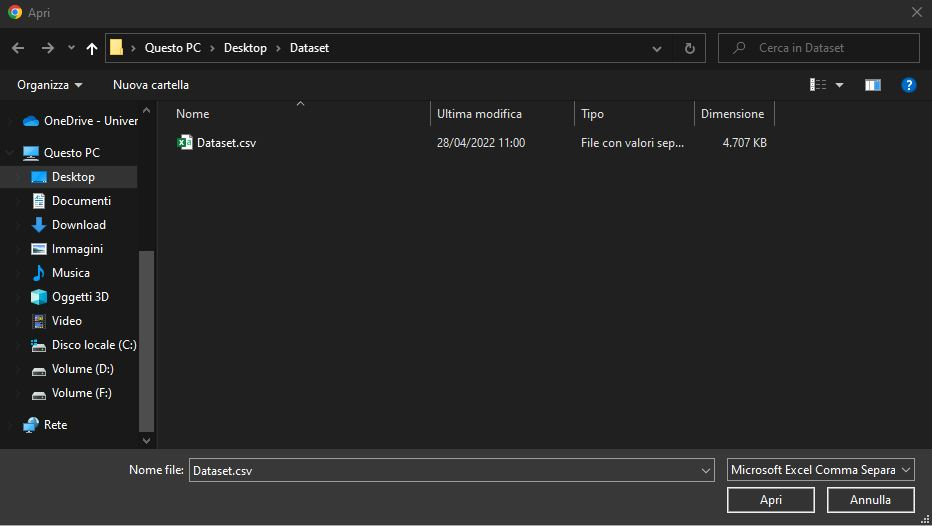
\includegraphics[width=1.0\textwidth]{BottoneDataset.jpg}
    \caption{Screenshot della finestra di dialogo per il caricamento del dataset}
\end{figure}

Dopo aver caricato il dataset comparirà una lista dei grafici disponibili.
Si potrà scegliere tra vari tipi di:
\begin{itemize}
  \item \textit{Scatter Plot};
  \item \textit{Parallel Coordinates};
  \item \textit{Sankey Diagram}.
\end{itemize}

\begin{figure}[H]
    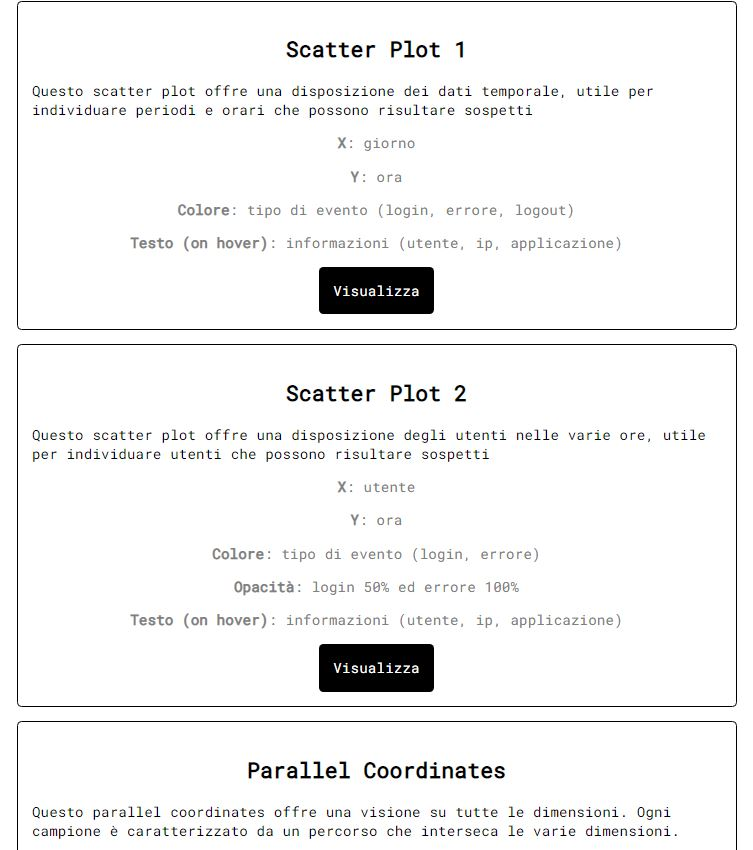
\includegraphics[width=1.0\textwidth]{ListaGrafici.jpg}
    \caption{Screenshot della lista dei grafici}
\end{figure}
Successivamente per visionare un grafico basterà premere il bottone "Visualizza".

\subsection{Carica sessione}
Cliccando su "Carica sessione" comparirà una finestra di dialogo che ci permetterà di caricare i dati di una sessione salvata in precedenza. Seleziona quindi il file desiderato e poi clicca su "Apri" per caricare il file.

\begin{figure}[H]
    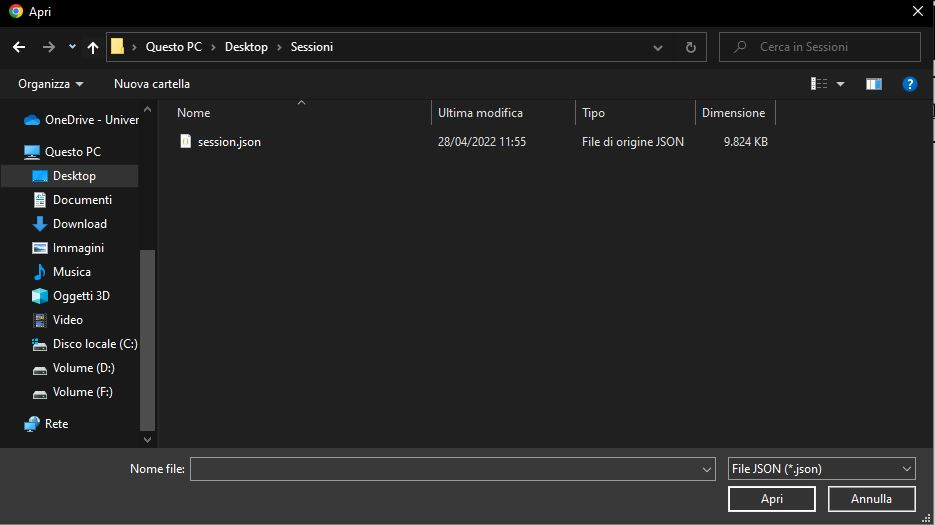
\includegraphics[width=1.0\textwidth]{BottoneSessione.JPG}
    \caption{Screenshot della finestra di dialogo per il caricamento della sessione}
\end{figure}

Dopo aver caricato la sessione nel sistema si potrà proseguire il lavoro da dove era stato salvato.

\begin{figure}[H]
    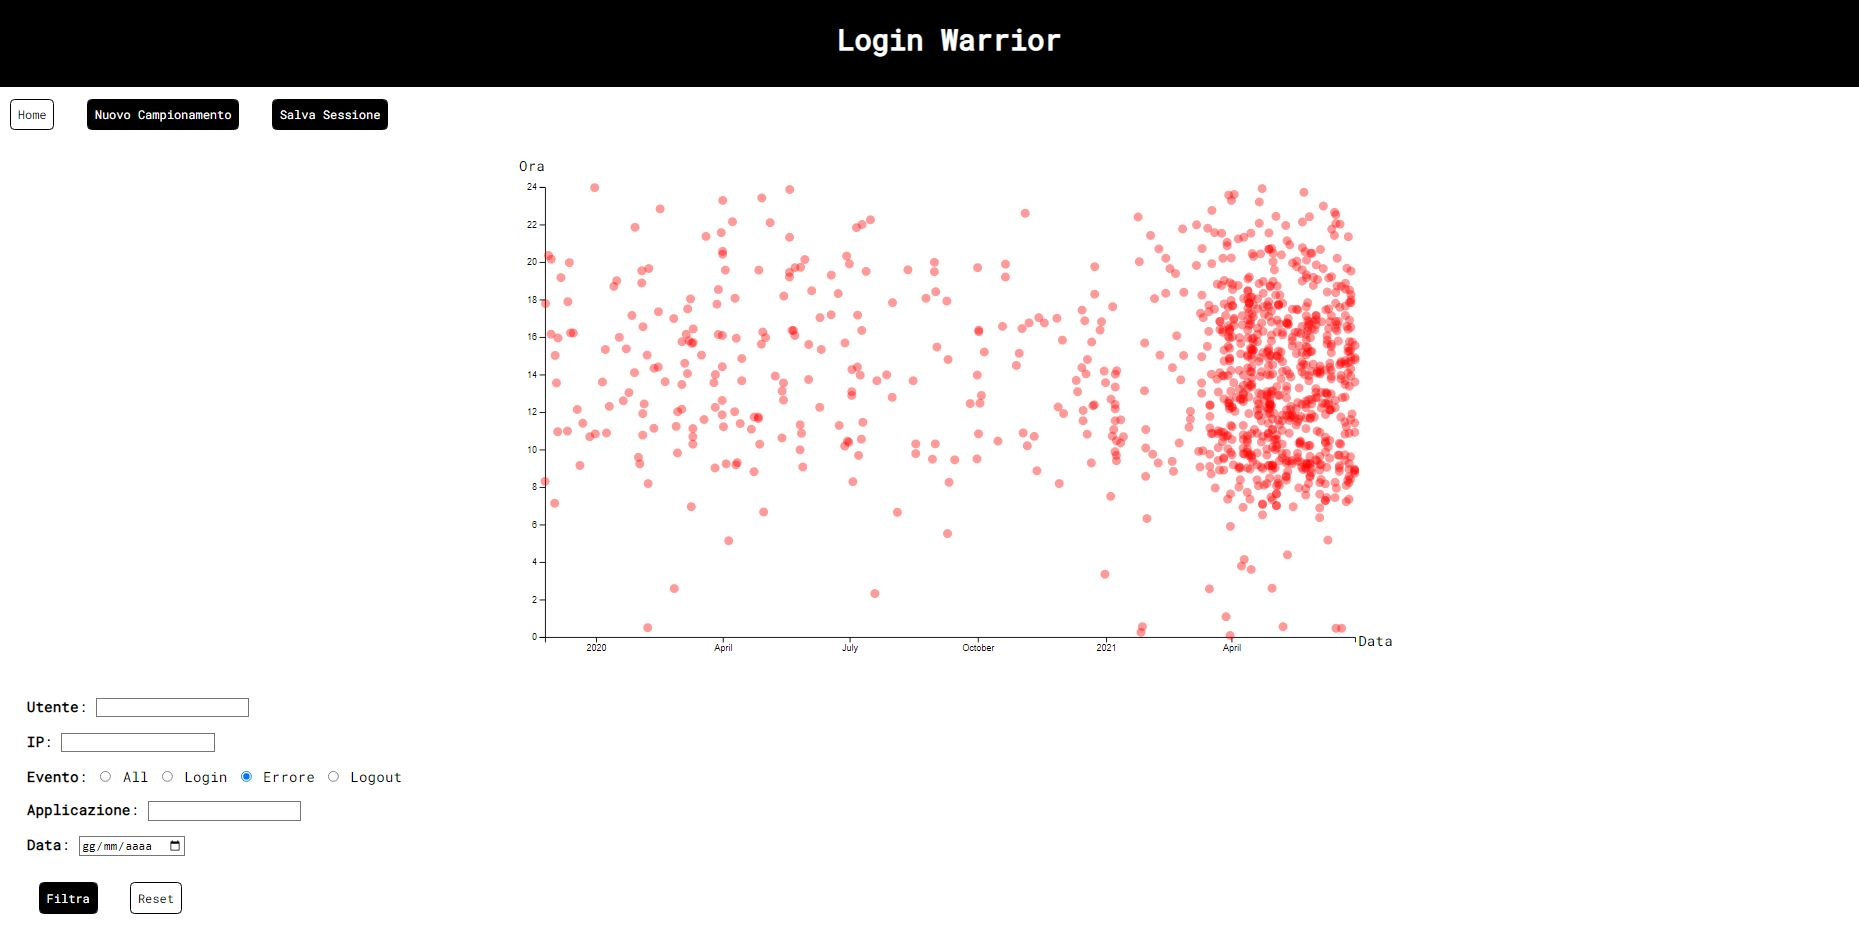
\includegraphics[width=1.0\textwidth]{CaricamentoSessione.JPG}
    \caption{Screenshot della sessione caricata}
\end{figure}

\section{Bottoni}
In ogni pagina di visualizzazione dei grafici, sono disponibili dei bottoni. Questi si trovano nell'estremo superiore sinistro della pagina.

\begin{figure}[H]
    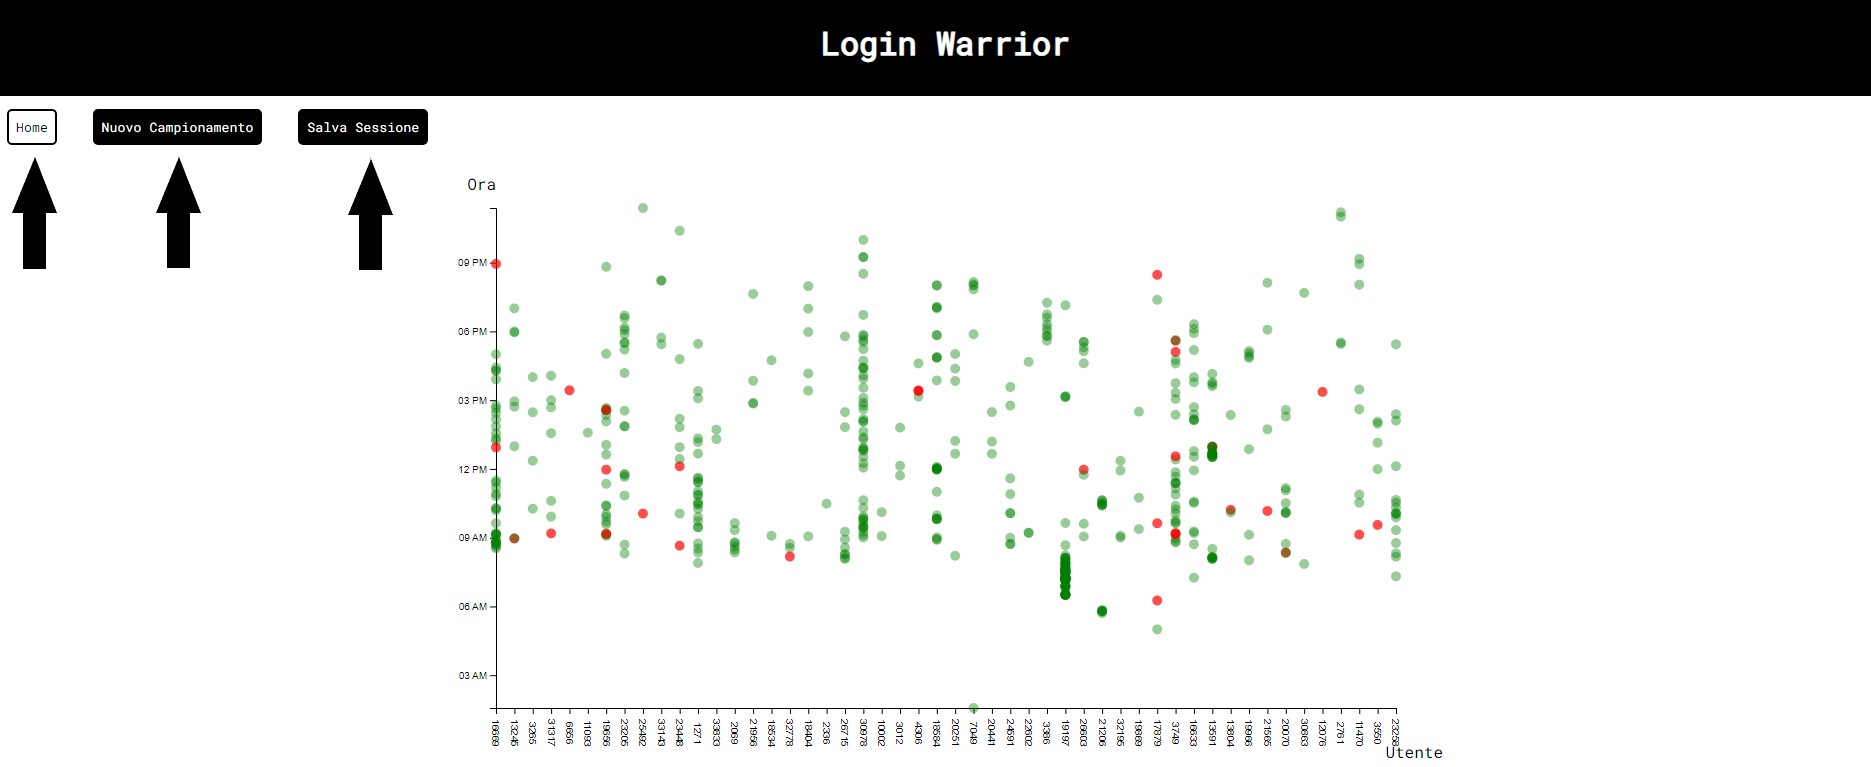
\includegraphics[width=1.0\textwidth]{Bottoni1.JPG}
    \caption{Screenshot che indica la posizione dei bottoni}
\end{figure}

\subsection{Bottone Home}
Questo bottone permette di ritornare alla Home in qualsiasi momento.

\subsection{Nuovo Campionamento}
Ogni grafico attua un algoritmo di campionamento dei dati del dataset per permettere all'utilizzatore di avere una buona visualizzazione delle informazioni (il numero di dati sennò potrebbe essere estremamente grande, quindi non gestibile).
Questo bottone permette di estrapolare ogni volta dei dati nuovi attraverso l'algoritmo di campionamento. Se il numero di dati del dataset è inferiore al numero massimo di dati che il grafico può visualizzare questo bottone non provoca cambiamenti.

\subsection{Salva Sessione}
Questo bottone permette di salvare la sessione corrente in tutti i suoi aspetti, compresi i filtri. Basterà premerlo per scaricare la sessione e averla a portata di file!

\section{Filtri}
In ogni grafico è possibile impostare dei filtri. Questi sono impostabili dall'estremo inferiore sinistro della pagina. Una volta inseriti i filtri desiderati occorre premere il bottone "Filtra" per applicarli. Per rimuovere i filtri invece occorre premere il bottone "Reset".

\begin{figure}[H]
    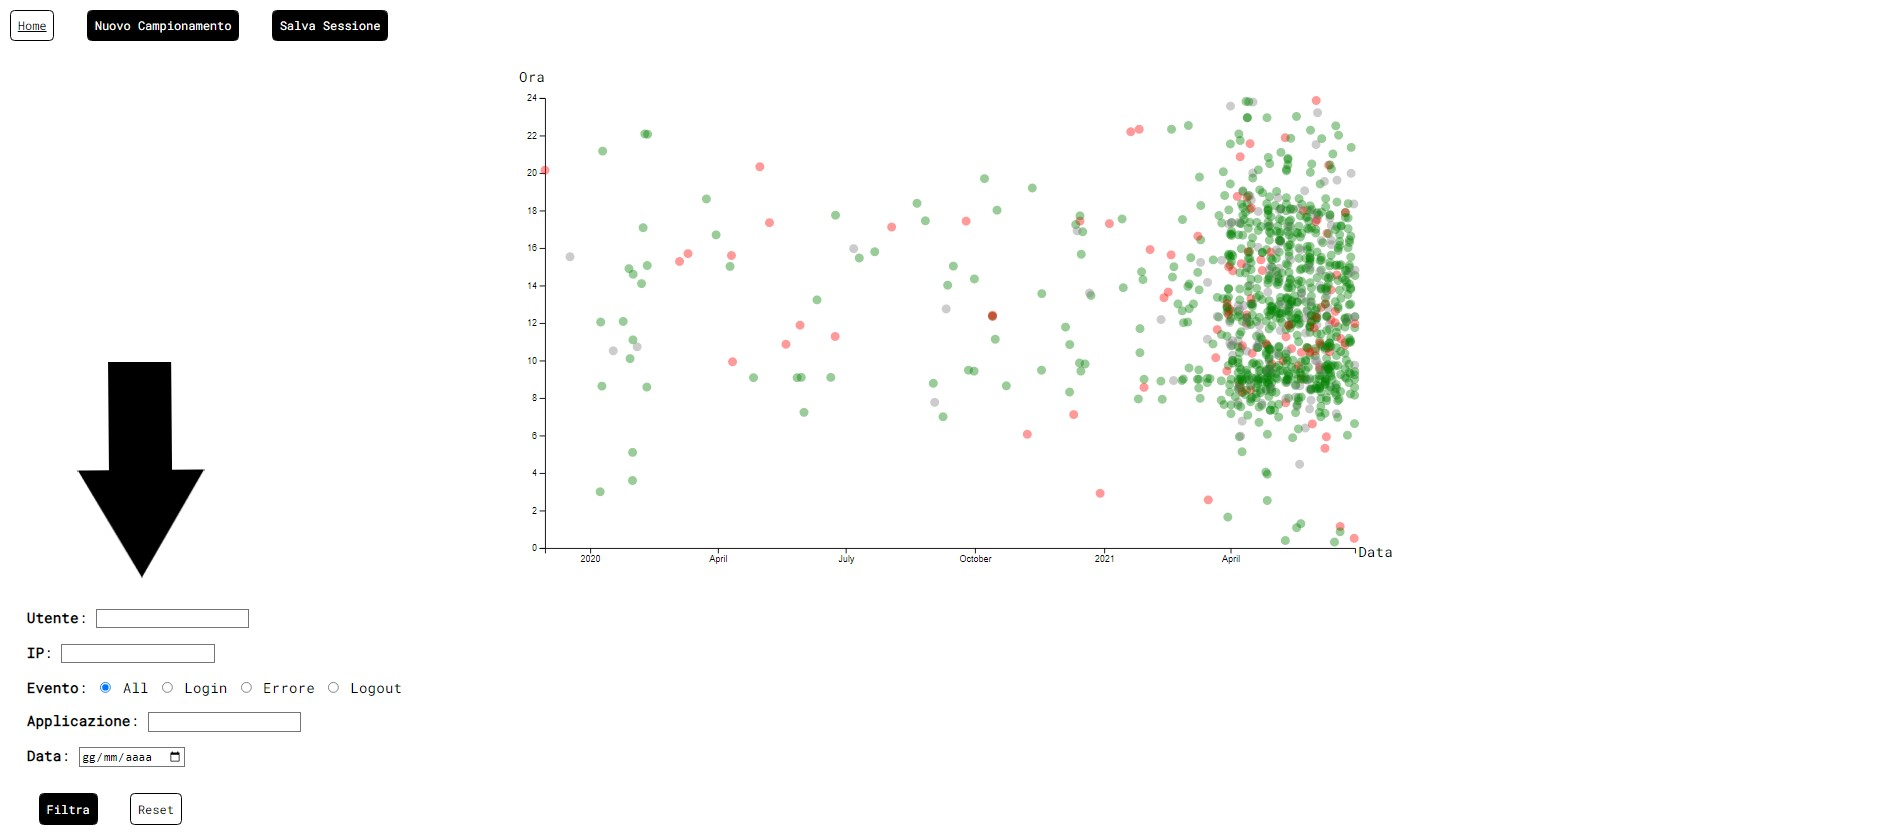
\includegraphics[width=1.0\textwidth]{Filtri.JPG}
    \caption{Screenshot che indica la posizione dei filtri}
\end{figure}

\subsection{Utente}
In questo campo è possibile inserire il numero di un utente in modo da filtrare il grafico secondo questo utente.

\subsection{Ip}
In questo campo è possibile inserire un indirizzo IP in modo da filtrare il grafico secondo questo IP.

\subsection{Evento}
Questo filtro permette di filtrare i dati secondo i vari tipi di evento, ovvero:
\begin{itemize}
  \item Login;
  \item Errore;
  \item Logout.
\end{itemize}

\subsection{Applicazione}
In questo campo è possibile inserire il nome di un'applicazione in modo da filtrare il grafico secondo questa applicazione.

\subsection{Data}
In questo campo è possibile inserire una data in modo da filtrare il grafico secondo questa particolare data.

\section{Scatter Plot}
Il grafico \textit{Scatter Plot} permette di visualizzare ogni azione degli utenti sotto forma di punti all'interno del piano cartesiano.
Ogni evento ha un colore differente per avere una più facile visualizzazione.
Il verde indica un login effettuato con successo, il rosso un errore e il grigio un logout.
Per visualizzare le informazioni di ogni evento si dovrà posizionare il cursore al di sopra del pallino scelto. Le informazioni disponibili sono:
\begin{itemize}
  \item Ip;
  \item Numero Utente;
  \item Tipologia di evento;
  \item Data;
  \item Applicazione da dove è stata compiuta l'azione.
\end{itemize}

\begin{figure}[H]
    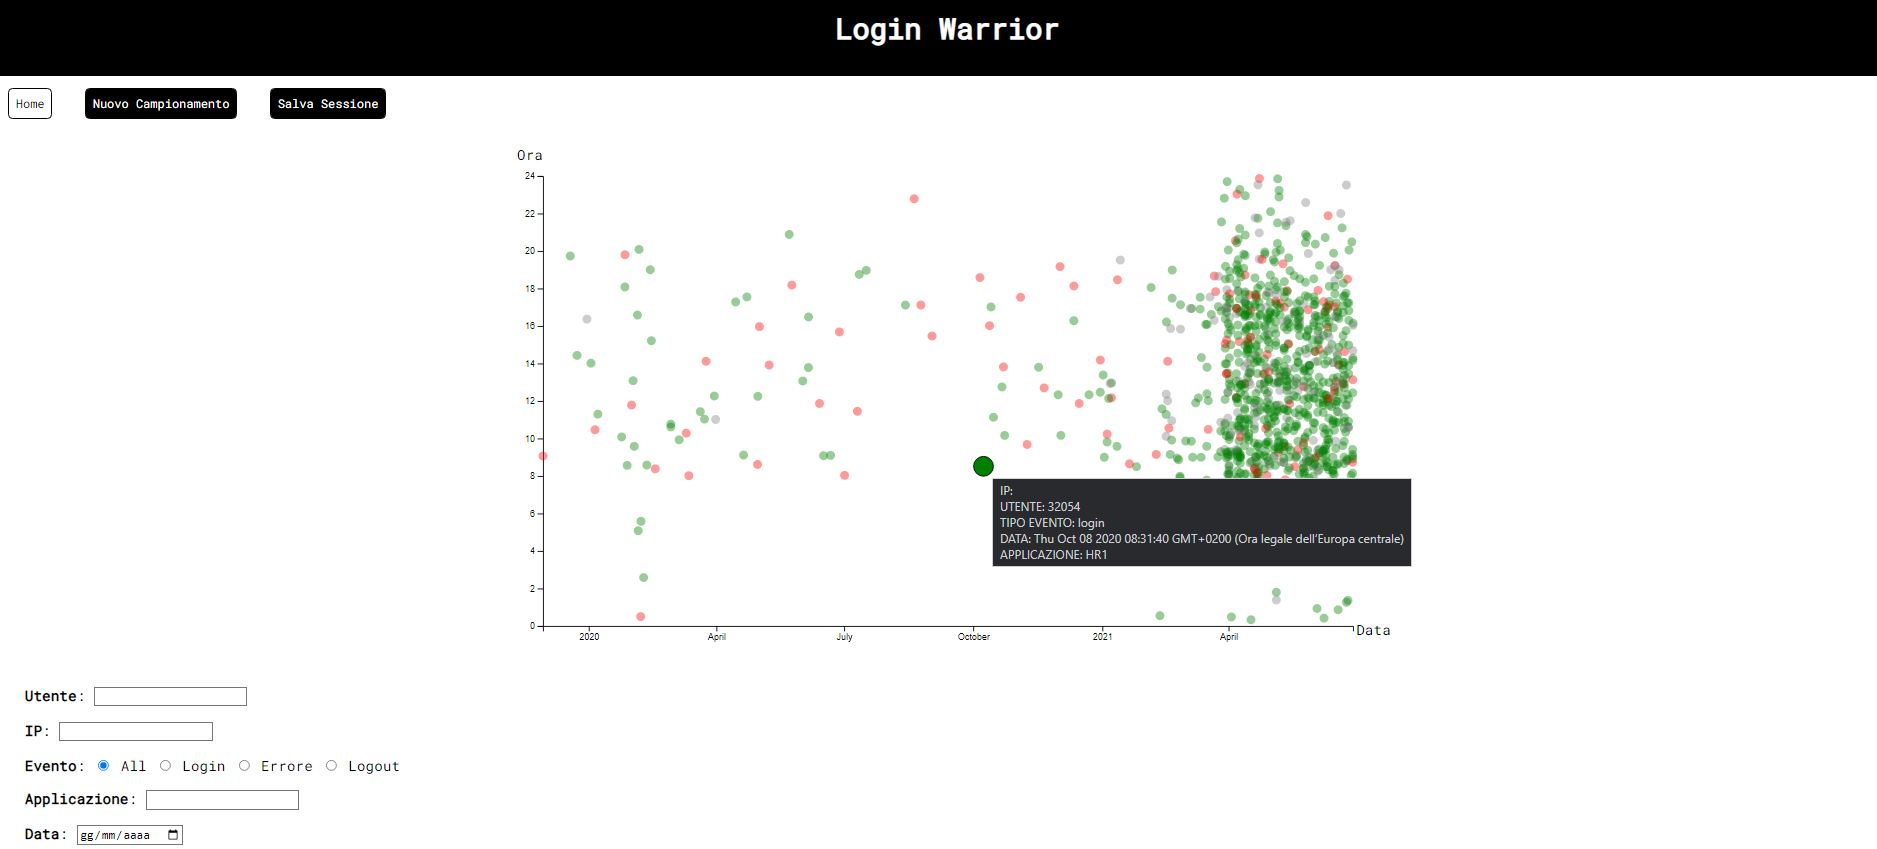
\includegraphics[width=1.0\textwidth]{VisualizzaInformazioni.JPG}
    \caption{Screenshot che mostra le informazioni di un punto}
\end{figure}

\section{Parallel Coordinates}
Il grafico \textit{Parallel Coordinates} permette di visualizzare ogni azione degli utenti sotto forma di linee.
Per visualizzare le informazioni di un particolare evento si dovrà posizionare il cursore al di sopra della linee scelta. Le informazioni disponibili sono:
\begin{itemize}
  \item Ip;
  \item Numero Utente;
  \item Tipologia di evento;
  \item Data;
  \item Applicazione da dove è stata compiuta l'azione.
\end{itemize}

\begin{figure}[H]
    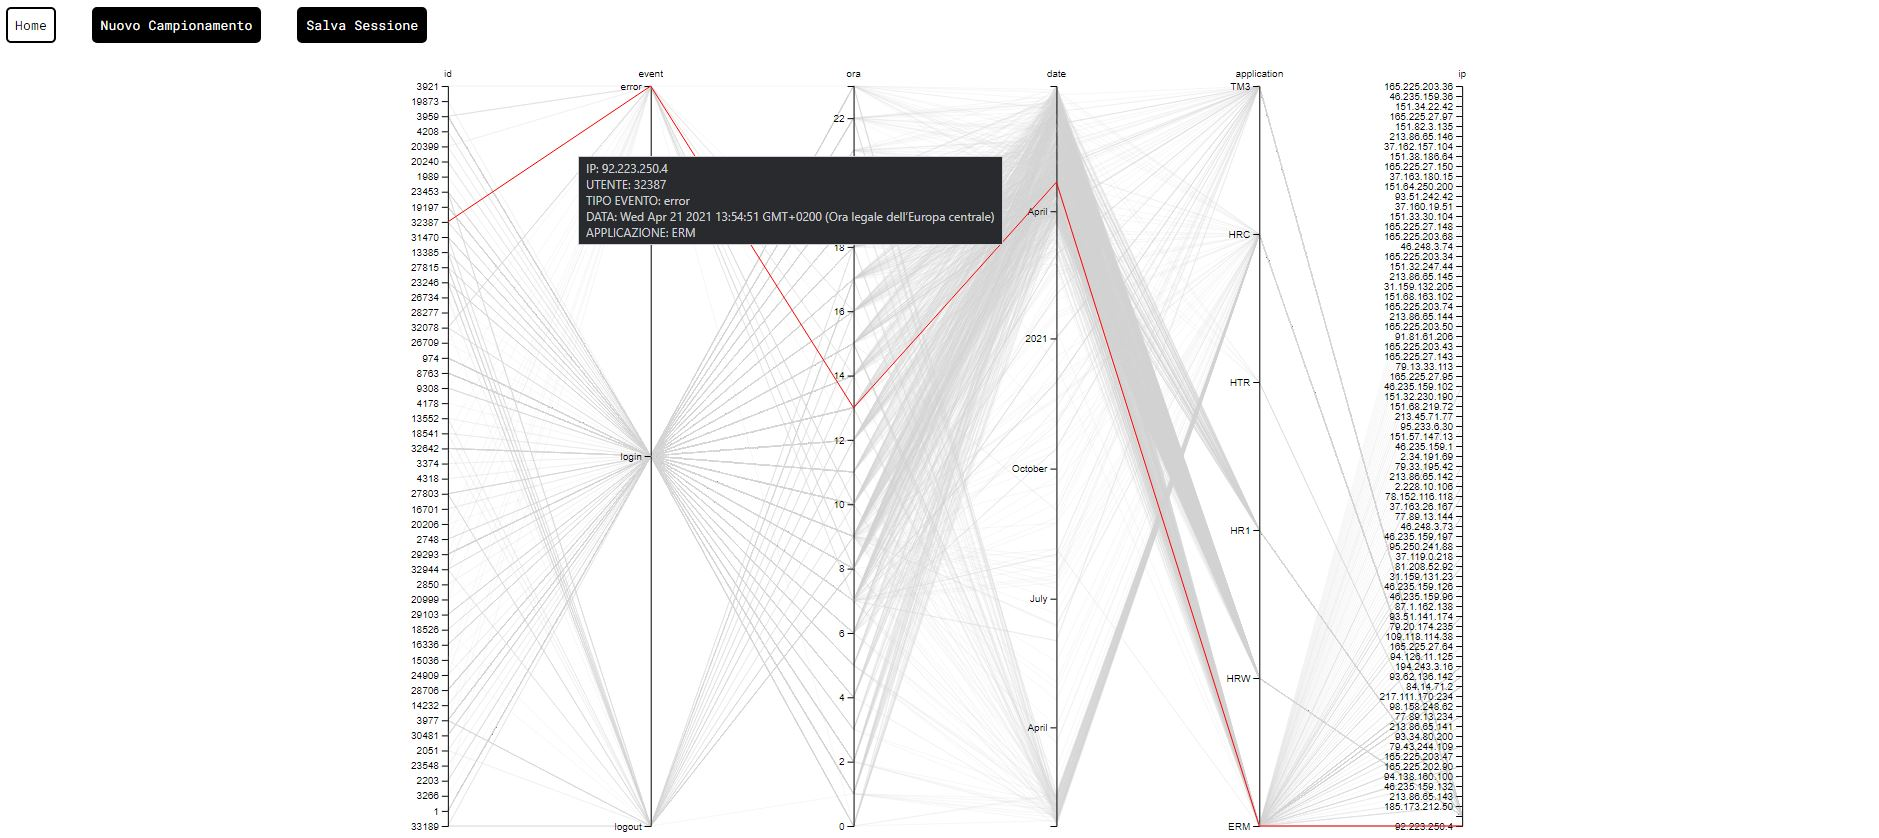
\includegraphics[width=1.0\textwidth]{Coordinates.JPG}
    \caption{Screenshot che mostra le informazioni di una linea}
\end{figure}

\section{Sankey Diagram}
Il grafico \textit{Sankey Diagram} permette di visualizzare gli eventi raggruppati in nodi.
È per esempio possibile visualizzare quanti login ci sono stati nel mese di Aprile nell'orario d'ufficio.
Per visualizzare il numero di dati che ogni nodo contiene basterà posizionare il cursore al di sopra del rettangolo colorato che indica i dati che ci interessano.

\begin{figure}[H]
    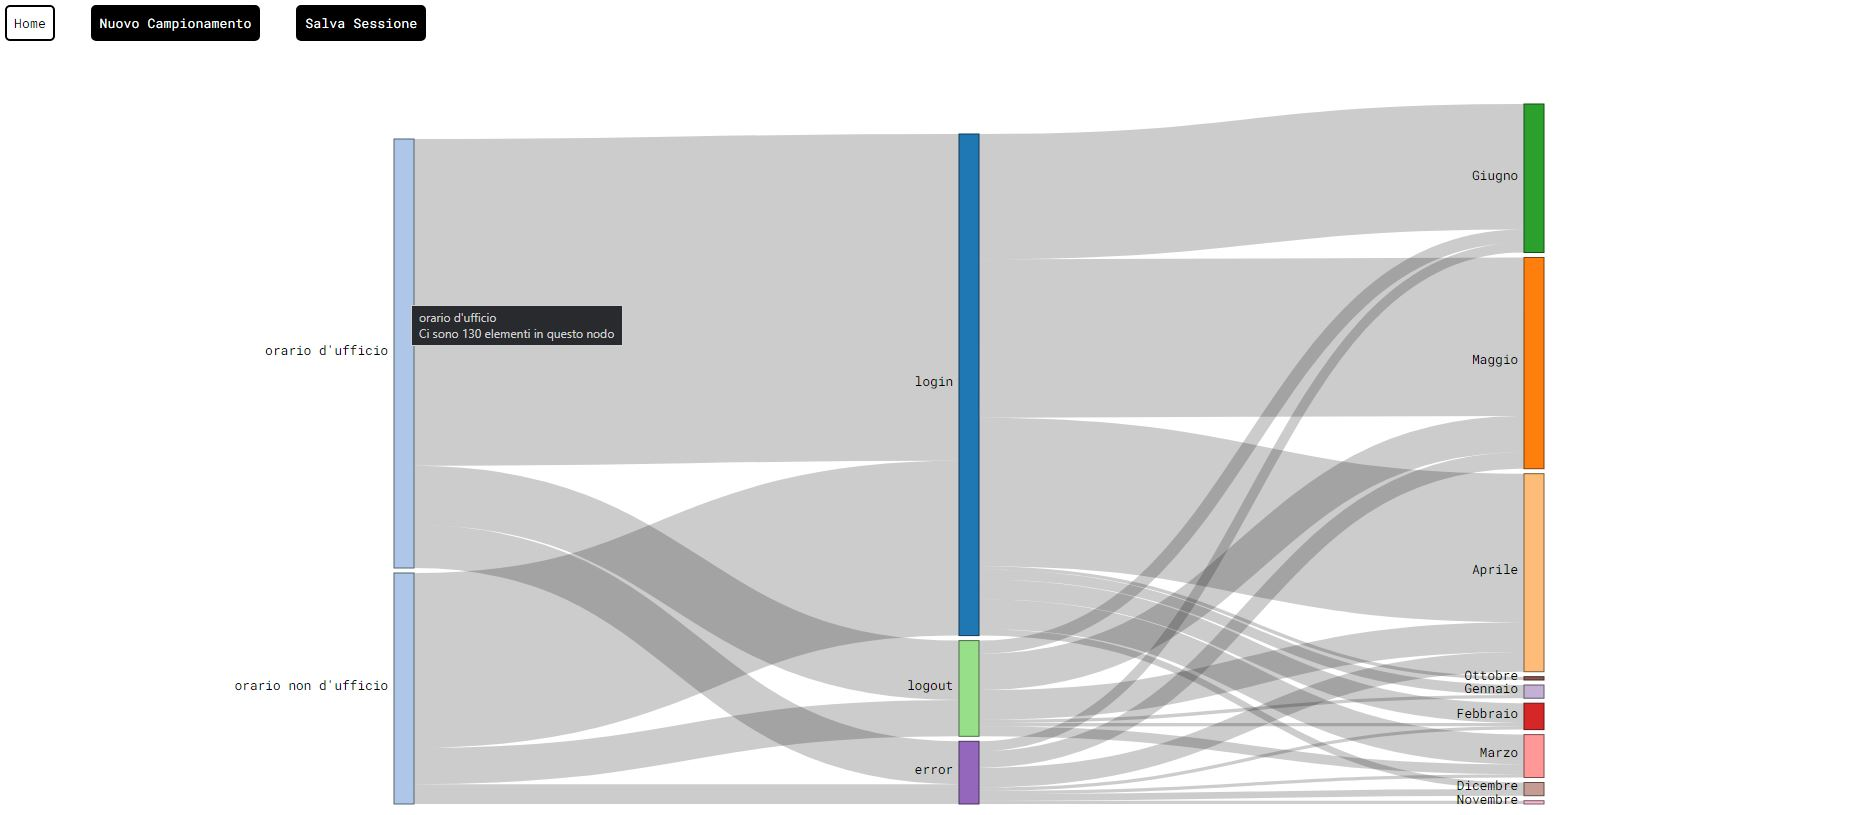
\includegraphics[width=1.0\textwidth]{Sankey.JPG}
    \caption{Screenshot che mostra le informazioni di un nodo}
\end{figure}
